\section{Generalities}
\subsection{Power}
All primary displays use electrical power from the secondary AC bus.
The displays are turned on by the yellow top-left button on the TI
(\cockpitref{fig:front-panel}{item:TI}).
In addition, displays are turned on at takeoff when RPM exceeds 90\%.

The HUD requires 40 seconds of preheating after AC power is available, before turning on.

\section{Head Up Display (HUD)}
\subsection{Overview}
\begin{figure}[!ht]
  \centering
  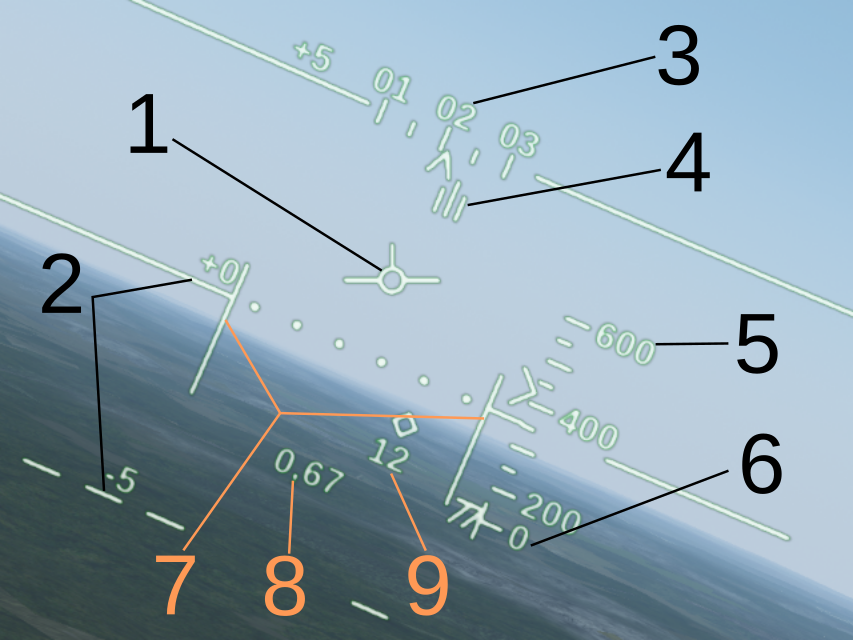
\includegraphics[width=0.7\textwidth]{images/displays/ja-hud-general.png}

  \begin{multicols}{2}
    \begin{enumerate}[nosep]
      \item \label{item:fpv} Flight path vector
      \item \label{item:horizon} Artificial horizon and pitch lines
      \item \label{item:heading} Heading scale
      \item \label{item:dest} Destination bearing
      \item \label{item:altitude} Altitude scale
      \item \label{item:rhm} Radar altimeter index and reference
      \item \label{item:altbars} Altitude bars
      \item \label{item:speed} Airspeed / Mach indicator
      \item \label{item:distance} Distance indicator
    \end{enumerate}
  \end{multicols}

  \caption{HUD overview}
  \label{fig:hud}
\end{figure}

\subsection{Navigation Mode}
\paragraph{Artificial Horizon (\cockpitref{fig:hud}{item:horizon})}
The artificial horizon and pitch scale provide an attitude reference.
The pitch scale consists of a line every 5 degrees.
Lines above the horizon are solid, lines below the horizon are dashed.
The artificial horizon itself is distinguished by six center dots.
Only the three pitch lines closes to the flight path vector are displayed.

\paragraph{Flight Path Vector (\cockpitref{fig:hud}{item:fpv})}
The FPV marker indicates the aircraft path direction relative to the ground.
Most of the HUD is centered around the FPV marker.

\paragraph{Heading Scale (\cockpitref{fig:hud}{item:heading})}
The heading scale is located above the FPV.
The fixed wedge index indicates aircraft track angle.
The second index consisting of 3 vertical lines
(\cockpitref{fig:hud}{item:dest}) indicates bearing to the next waypoint.

\paragraph{Altitude Scale (\cockpitref{fig:hud}{item:altitude})}
The altitude scale is located right of the FPV.
The fixed wedge index indicates aircraft altitude.
At low altitude the scale zooms in,
allowing to read the altitude more precisely for low level flight.

When the radar altimeter is active and in range,
the altitude 0 mark is displayed just below the altitude scale
(\cockpitref{fig:hud}{item:rhm}).
The radar altitude index, consisting of two wedges, can be read against this mark.
This can be used to set the altimeter QFE in flight.

\paragraph{Altitude Bars (\cockpitref{fig:hud}{item:altbars})}
The two altitude bars indicate the reference altitude
(also called commanded altitude) relative to the current altitude.

The top of the altitude bars represents commanded altitude,
while the artificial horizon represents current altitude.
If the top of the bars is on the horizon, the aircraft is at the commanded altitude.
If the top of the bars is above (resp.\ below) the horizon,
the aircraft is below (resp.\ above) the commanded altitude.

Altitude bars are only displayed below 1000m.
When autopilot altitude hold is active, boxes are displayed together with the altitude bars.

\paragraph{Airspeed / Mach Indicator (\cockpitref{fig:hud}{item:speed})}
Digital airspeed is displayed below the FPV,
with a minimum of 75km/h and a precision of 5km/h
(40kts and 1kts respectively in imperial units mode).
Above M0.5, airspeed is replaced by a Mach indicator.

\paragraph{Distance Indicator (\cockpitref{fig:hud}{item:distance})}
Displays digital distance to the next waypoint.
